\chapter{Parâmetros, fontes e proveniência}
\label{app:parametros}

Este apêndice consolida, em formato de consulta, os grupos de insumos e a lógica de proveniência usados no relatório. Sua função é apoiar a leitura do Capítulo~\ref{ch:metodologia} e separar, para cada parâmetro, fonte, uso e limite de interpretação.

\section{Inventário resumido de fontes}
\label{sec:app-inventario-fontes}

A Tabela~\ref{tab:app-fontes-proveniencia} resume as famílias de fontes e artefatos derivados citadas na metodologia. Sempre que uma fonte tiver data, recorte, cobertura ou fronteira limitada, essa limitação deve acompanhar qualquer interpretação de resultado.

\begingroup
\footnotesize
\setlength{\LTleft}{0pt}
\setlength{\LTright}{0pt}
\setlength{\tabcolsep}{4pt}
\renewcommand{\arraystretch}{1.15}
\begin{longtable}{L{0.20\textwidth}L{0.25\textwidth}L{0.25\textwidth}L{0.22\textwidth}}
\caption{Inventário resumido de fontes, usos e limites de interpretação.}
\label{tab:app-fontes-proveniencia}\\
\toprule
Fonte ou origem & Artefato ou dado derivado & Uso metodológico & Limite de interpretação \\
\midrule
\endfirsthead
\toprule
Fonte ou origem & Artefato ou dado derivado & Uso metodológico & Limite de interpretação \\
\midrule
\endhead
ANTAQ & Viagens, sequência de escalas, movimentações de carga, massa, TEU e número IMO. & Reconstrução da carga a bordo, dos subtrechos e dos corredores observados entre pares ordenados de portos. & Base observada de 2025; não garante disponibilidade futura de serviço, frequência ou slot.\\
EU MRV & Intensidade por trabalho de transporte, período de referência, IMO, classe e tipo de navio. & Correspondência exata por IMO e estatísticas robustas de fallback por classe ou tipo. & Proxy europeu; pode não representar integralmente a frota brasileira.\\
OpenRouteService & Distâncias rodoviárias, geocodificação e metadados de rota. & Rotas terrestres da alternativa direta, \emph{pre-carriage} e \emph{on-carriage}. & Rota modelada por API, não viagem GPS observada nem rota comercial contratual.\\
LocationIQ & Saídas alternativas de geocodificação ou roteamento quando configuradas. & Fallback de resolução de localidade ou rota. & Deve permanecer rastreável e não substituir silenciosamente a fonte principal.\\
Ship \& Bunker / VLSFO Santos & Preço processado de combustível marítimo. & Insumo do proxy de custo operacional marítimo. & Fonte volátil e sensível à data; Santos pode funcionar apenas como proxy.\\
CSV de diesel processado & Preços de diesel por UF usados pelo avaliador. & Insumo de custo de combustível rodoviário. & Custo permanece proxy operacional; data e método de extração devem continuar visíveis quando disponíveis.\\
SeaMatrix schema 3 e referências de distância & Intensidade representativa do par, corredores observados, subtrechos, distâncias e metadados de proveniência. & Definição separada da estatística de intensidade e da geometria usada no cenário. & \texttt{haversine\_fallback} é triagem, não rota marítima validada.\\
Literatura e notas técnicas de portos & Valores observados, média ponderada, padrão documentado ou indisponibilidade. & Componentes de operações portuárias e \emph{hoteling}. & Dados ausentes não devem ser interpretados como zero silencioso.\\
Presets de caminhão e fatores & Consumo rodoviário e fatores implementados. & Emissões operacionais \ttw{} de \cooe{} nas pernas terrestres. & Fonte, unidade e fronteira devem permanecer explícitas.\\
Prof. Dr. Gustavo Costa & Pares OD, rotas, fatores ou planilhas usados em benchmark. & Referência externa de plausibilidade e direção. & Não é verdade de referência, nem alvo de reprodução calibrada.\\
\bottomrule
\end{longtable}
\endgroup

\section{Parâmetros e regras do estimador marítimo}
\label{sec:app-parametros-maritimos}

A Tabela~\ref{tab:app-parametros-maritimos} consolida as regras que transformam as observações ANTAQ e os indicadores EU MRV na intensidade marítima aplicada pelo sistema. Os parâmetros descrevem decisões determinísticas e reprodutíveis do modelo.

\begingroup
\footnotesize
\setlength{\LTleft}{0pt}
\setlength{\LTright}{0pt}
\setlength{\tabcolsep}{4pt}
\renewcommand{\arraystretch}{1.15}
\begin{longtable}{L{0.22\textwidth}L{0.29\textwidth}L{0.25\textwidth}L{0.16\textwidth}}
\caption{Parâmetros e regras da intensidade marítima direcional.}
\label{tab:app-parametros-maritimos}\\
\toprule
Elemento & Regra & Metadado associado & Unidade ou valor \\
\midrule
\endfirsthead
\toprule
Elemento & Regra & Metadado associado & Unidade ou valor \\
\midrule
\endhead
Elegibilidade same-OD & Considerar a viagem quando o porto de origem aparece antes do porto de destino na sequência; incluir ligação direta e qualquer número de escalas intermediárias. & Contagens de viagens candidatas, diretas e multiescala; caminhos observados. & Uma observação por viagem e par.\\
Carga inicial & Aplicar o menor deslocamento inicial que mantém não negativa a carga acumulada em toda a sequência. & \codecell{minimum\_nonnegative\_prefix\_offset} e estado da reconstrução. & t e TEU.\\
Trabalho de transporte & Somar carga a bordo vezes distância em todos os subtrechos entre origem e destino. & \codecell{observed\_transport\_work\_tnm}. & \(\mathrm{t\,nm}\).\\
Intensidade exata & Usar o valor positivo do período EU MRV mais recente para o IMO da viagem. & Fonte \codecell{eu\_mrv\_imo\_latest}; período e IMO. & \(\mathrm{g/(t\,nm)}\).\\
Fallback por classe & Usar média aparada simétrica de 1\% em cada cauda, excluindo valores abaixo do percentil 1 e acima do percentil 99; usar mediana se essa estatística estiver indisponível. & Classe, estatística, amostra e regra de outlier. & \(\mathrm{g/(t\,nm)}\).\\
Fallback por tipo & Ordenar os valores positivos mais recentes por IMO e remover \(\lfloor0{,}01n\rfloor\) de cada cauda antes da média; usar mediana quando a amostra não permite corte. & Tipo, valor-padrão quando aplicável, amostra bruta/retida, limites e excluídos. & \(\mathrm{g/(t\,nm)}\).\\
Valor exato e outliers & Não aparar a intensidade de um IMO individual; aplicar o tratamento robusto somente às distribuições de fallback. & Nível da fonte e política de outlier. & Regra categórica.\\
Intensidade do par & Usar a mediana das intensidades das viagens ponderada pelo trabalho de transporte de todas as viagens resolvidas e de todos os corredores do par. & Método, escopo, peso, fonte e contagens efetivas. & \(\mathrm{g/(t\,nm)}\).\\
Empate na mediana & Escolher a primeira intensidade ordenada cuja massa acumulada atinge 50\% do peso positivo. & Regra da função de distribuição inversa inferior. & Regra determinística.\\
Trabalho nulo & Excluir peso nulo quando houver pesos positivos; se todos forem nulos, usar mediana não ponderada das intensidades resolvidas. & Contagens de peso positivo/nulo e fonte específica para o caso nulo. & Regra determinística.\\
Seleção do corredor & Priorizar corredor direto observado e, dentro da categoria aplicável, a menor distância; usar o caminho apenas para sequência e distância. & \codecell{direct\_first\_then\_shortest\_distance\_km}, corredor e alternativas. & Caminho geométrico.\\
Consumo do cenário & Aplicar a intensidade do par à massa da remessa e à soma das distâncias dos subtrechos selecionados. & Intensidade aplicada, intensidade observada do corredor e modo de cálculo. & kg de combustível.\\
Contrato do artefato & Exigir schema marítimo 3, data de geração e campos de intensidade do par em cada estatística direcional. & Versão do parser, schema, entradas e cobertura. & Versão 3.\\
\bottomrule
\end{longtable}
\endgroup

\section{Hierarquia de proveniência}
\label{sec:app-hierarquia-proveniencia}

A Figura~\ref{fig:proveniencia-hierarquia} sintetiza a hierarquia de proveniência usada para interpretar os principais insumos do modelo.

\begin{figure}[htbp]
\centering
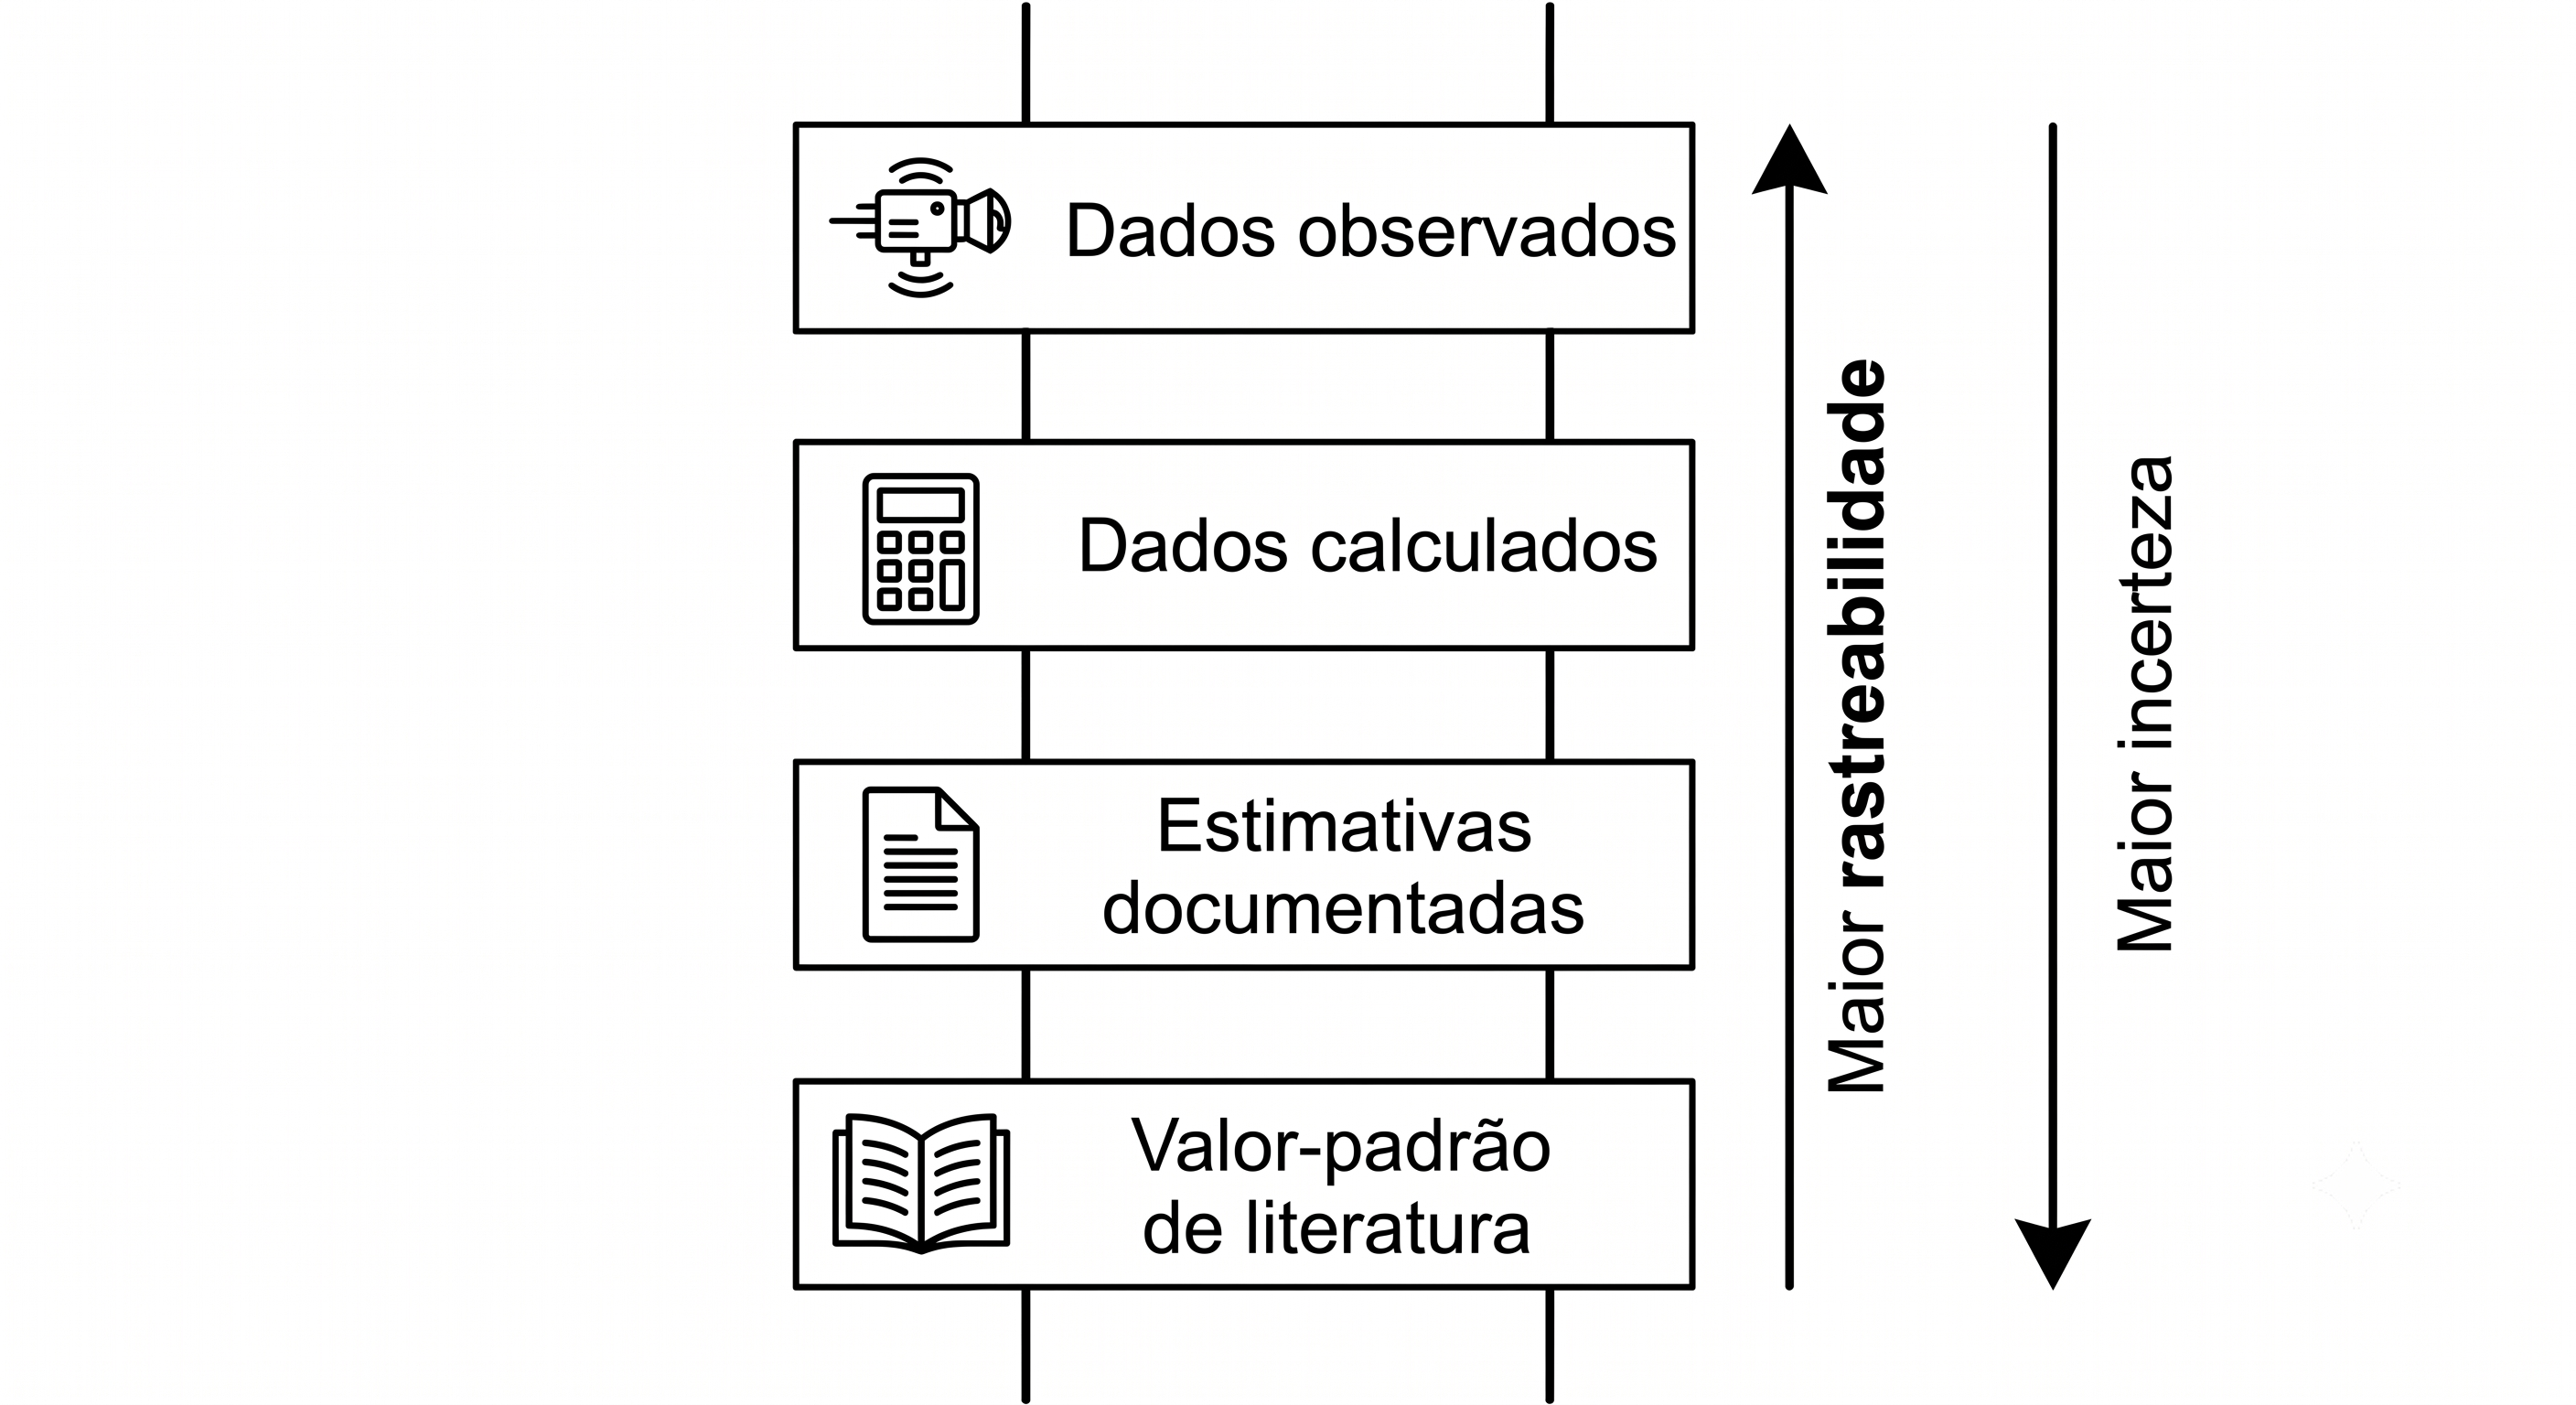
\includegraphics[width=0.85\textwidth]{images/figura_A_1.png}
\caption{Hierarquia de proveniência adotada para classificação das fontes de dados, priorizando maior rastreabilidade e explicitando o aumento de incerteza associado a estimativas e valores-padrão de literatura.}
\label{fig:proveniencia-hierarquia}
\end{figure}

A Tabela~\ref{tab:app-proveniencia-distancias} detalha a hierarquia aplicada às distâncias e aos componentes de rota. A leitura mais forte depende de referência específica para o par e para a fronteira analisada; a leitura mais fraca deve permanecer como triagem, lacuna ou sensibilidade.

\begin{table}[htbp]
\centering
\small
\caption{Hierarquia de proveniência para distâncias e componentes de rota.}
\label{tab:app-proveniencia-distancias}
\begin{tabularx}{\textwidth}{L{0.24\textwidth}Y Y}
\toprule
Proveniência & Uso metodológico & Limite de interpretação \\
\midrule
Roteamento rodoviário/cache & Distância terrestre para rota direta, \emph{pre-carriage} e \emph{on-carriage}. & Não é trajetória GPS medida nem rota comercial efetivamente usada.\\
\codecell{seamatrix} & Distância marítima matricial para par de portos aplicável. & Não comprova escala, frequência, serviço ou contrato.\\
\codecell{external\_reference} & Referência documentada para o par de portos do cenário. & Só vale para o par e a unidade informados.\\
\codecell{manual\_override} & Substituição documentada ou entrada forçada para cenário rastreado. & Deve permanecer explícita como decisão metodológica.\\
\codecell{haversine\_fallback} & Aproximação geométrica quando falta fonte melhor. & Triagem; não valida rota marítima operacional.\\
\codecell{unavailable} & Ausência de valor defensável. & Não deve ser tratado como zero silencioso.\\
\bottomrule
\end{tabularx}
\end{table}

\section{Operações portuárias e hoteling}
\label{sec:app-portops-hoteling}

Operações portuárias e \emph{hoteling} têm importância metodológica porque a alternativa multimodal não é apenas uma perna marítima. Quando o cenário aplica a intensidade EU MRV por trabalho de transporte, o indicador anual é tratado como abrangente do consumo reportado pelo navio e o \emph{hoteling} não é somado separadamente, evitando dupla contagem. A Tabela~\ref{tab:app-portops-proveniencia} registra a regra de interpretação para os componentes representados separadamente e para os níveis de proveniência usados nesses componentes.

\begin{table}[htbp]
\centering
\small
\caption{Proveniência de operações portuárias e hoteling.}
\label{tab:app-portops-proveniencia}
\begin{tabularx}{\textwidth}{L{0.25\textwidth}Y Y}
\toprule
Proveniência & Uso permitido & Cautela \\
\midrule
\codecell{observed} & Usar como dado observado para porto, chamada ou condição documentada. & Ainda não equivale a inventário terminal-específico completo.\\
\codecell{estimated\_port\_average} & Usar como média ponderada quando observações específicas sustentam a estimativa. & Menor confiança que observação direta do caso.\\
\codecell{literature\_default} & Usar como padrão documentado quando não há valor observado defensável. & Deve ser identificado como aproximação.\\
\codecell{unavailable} & Registrar ausência de dado. & Não converter ausência em zero emissões, zero custo ou zero tempo.\\
\bottomrule
\end{tabularx}
\end{table}
